\documentclass{article}

\usepackage{graphicx}
\usepackage{tikz}
\usepackage{tikzsymbols}
\usetikzlibrary{calc,patterns,shapes.geometric}
\pagestyle{empty}
\usepackage[margin=0pt]{geometry}
\geometry{papersize={14in,12in}}

\def\centerarc[#1](#2)(#3:#4:#5){\draw[#1] ($(#2)+({#5*cos(#3)},{#5*sin(#3)})$) arc (#3:#4:#5);}

\begin{document}
	\begin{figure}
		\centering
		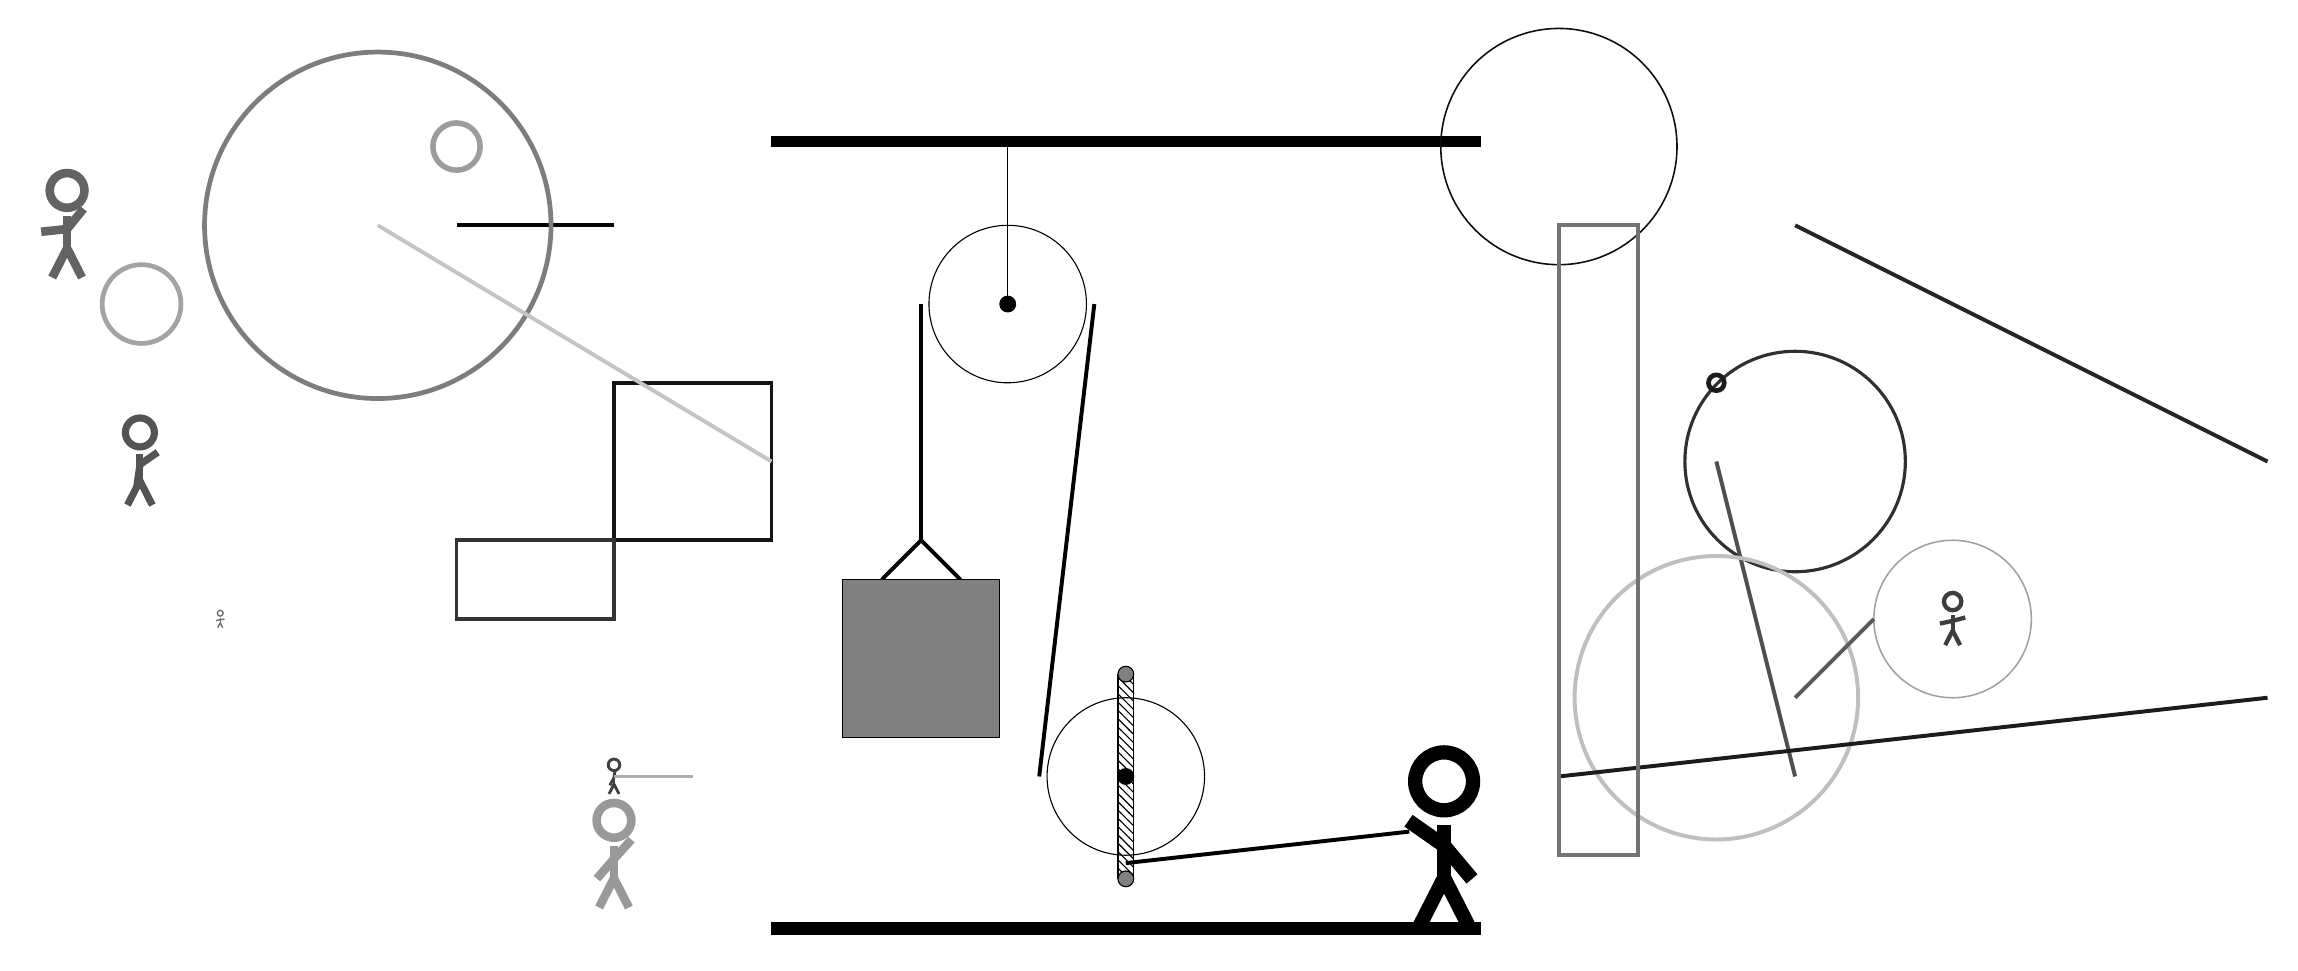
\begin{tikzpicture}
			%%%%% START %%%%%
			
			\draw[fill=black] (-2, 10) rectangle (7, 10.125);
			
			\draw (1, 8) circle (1);
			\draw[fill=black] (1, 8) circle (0.1);
			\draw (1, 10) -- (1, 8);
			
			\node[line width=0.2mm, color=black!75] at (-4, 2) {\Strichmaxerl[2][61][82]};
			
			\draw[line width=0.5mm, color=black!85](11, 9) -- (17, 6);
			\node[line width=0.2mm, color=black!56] at (-9, 4) {\Strichmaxerl[1][13][5]};
			\draw [line width=0.2mm, color=black!37](13, 4) circle (1.0);
			\draw[line width=0.5mm, color=black!32](-4, 2) -- (-3, 2);
			\node[line width=0.3mm, color=black!61] at (-11, 9) {\Strichmaxerl[6][6][51]};
			\node[line width=0.6mm, color=black!67] at (-10, 6) {\Strichmaxerl[5][82][35]};
			\draw [line width=0.4mm, color=black!81](11, 6) circle (1.4);
			\draw [line width=0.6mm, color=black!89](10, 7) circle (0.1);
			
			\draw[line width=0.5mm, color=black!99](-4, 9) -- (-6, 9);
			
			\draw [line width=0.6mm, color=black!51](-7, 9) circle (2.2);
			
			\draw[line width=0.5mm, color=black!92] (-4, 5) rectangle (-2, 7);
			\draw[line width=0.5mm, color=black!69](10, 6) -- (11, 2);
			\draw [line width=0.7mm, color=black!39](-6, 10) circle (0.3);
			\draw [line width=0.5mm, color=black!25](10, 3) circle (1.8);
			\node[line width=0.4mm, color=black!40] at (-4, 1) {\Strichmaxerl[6][49][48]};
			
			\draw[line width=0.5mm, color=black!23](-2, 6) -- (-7, 9);
			\draw [line width=0.2mm, color=black!95](8, 10) circle (1.5);
			\draw[line width=0.5mm, color=black!80] (-4, 4) rectangle (-6, 5);
			
			\node[line width=0.7mm, color=black!76] at (13, 4) {\Strichmaxerl[3][12][15]};
			\draw[line width=0.5mm, color=black!89](8, 2) -- (17, 3);
			
			\draw [line width=0.6mm, color=black!36](-10, 8) circle (0.5);
			\draw[line width=0.5mm, color=black!64](11, 3) -- (12, 4);
			\draw[line width=0.5mm, color=black!55] (9, 1) rectangle (8, 9);
			
			\draw[fill=white](2.5, 2.0) circle (1);
			\draw[fill=black] (2.5, 2.0) circle (0.1);
			\draw[pattern=north west lines, pattern color=black] (2.4, 3.3) rectangle (2.6, 0.7);
			\draw[fill=black!50] (2.5, 3.3) circle (0.1);
			\draw[fill=black!50] (2.5, 0.7) circle (0.1);
			
			\draw[line width=0.5mm] (-0.6, 4.5) -- (-0.1, 5.0) -- (0.4, 4.5);
			\draw[fill=black!50] (-1.1, 4.5) rectangle (0.9, 2.5);
			
			\draw[line width=0.5mm] (-0.1, 8) -- (-0.1, 5.0);
			\centerarc[line width=0.5mm](1, 8)(0:180:1.1);
			\draw[line width=0.5mm](2.1, 8) -- (1.4, 2.0);
			\centerarc[line width=0.5mm](2.5, 2.0)(180:270:1.1);
			\draw[line width=0.5mm](2.5, 0.9) -- (6.1, 1.3);
			
			\node at (6.5, 1.2) {\Strichmaxerl[10][-35][-50]};
			
			\draw[fill=black] (-2, 0) rectangle (7, 0.15);
			
			%%%%% END %%%%%
		\end{tikzpicture}
	\end{figure}	
\end{document}